\documentclass[12pt]{article}
\usepackage[margin=2cm]{geometry} 
\usepackage{titling}
\usepackage{graphicx}
\usepackage{float}
\usepackage[hidelinks]{hyperref}
\usepackage[english]{babel}
\usepackage{subcaption}

\setlength\parindent{0pt}
\setlength{\parskip}{1em}
\setlength{\droptitle}{-2cm}

\title{User instructions AR Sandbox (for internal use)}
\author{Università della Svizzera italiana}
\date{Version \today}


\begin{document}
\maketitle
\tableofcontents
\newpage


\section{Installation}\label{installation}

\subsection{Components}

\begin{itemize}
	\item PC
	\item Long DVI cable and 2 3-phase power cables
	\item \textit{projectiondesign F10 AS3D wide} projector
	\item Kinect v2 and adapter
	\item 4 M6x50 screws
\end{itemize}


\subsection{Assembly}

\begin{enumerate}
	\item Connect the power cables and the DVI (MONO 2D entrance) to the projector
	\item Assemble the projector on the support by using 4 screws and let the cables go through the opening
	\item Assemble the Kinect on the support and let the cable go through the opening
	\item Connect the power cables and the DVI to the PC
	\item Connect the Kinect to its adapter. Then connect the adapter to the power supply and to a USB 3.0 port (blue) in the PC
\end{enumerate}

\begin{figure}[H]
	\centering
	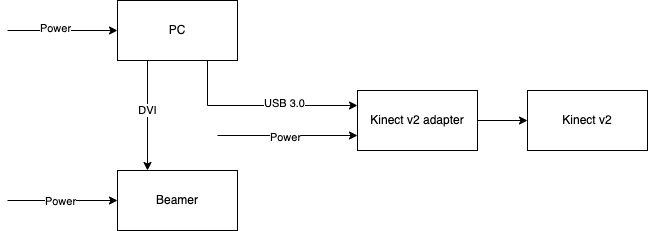
\includegraphics[width=0.9\textwidth]{img/cablesScheme.png}
	\caption*{Cables scheme}
\end{figure}

\begin{figure}[H]
	\centering
	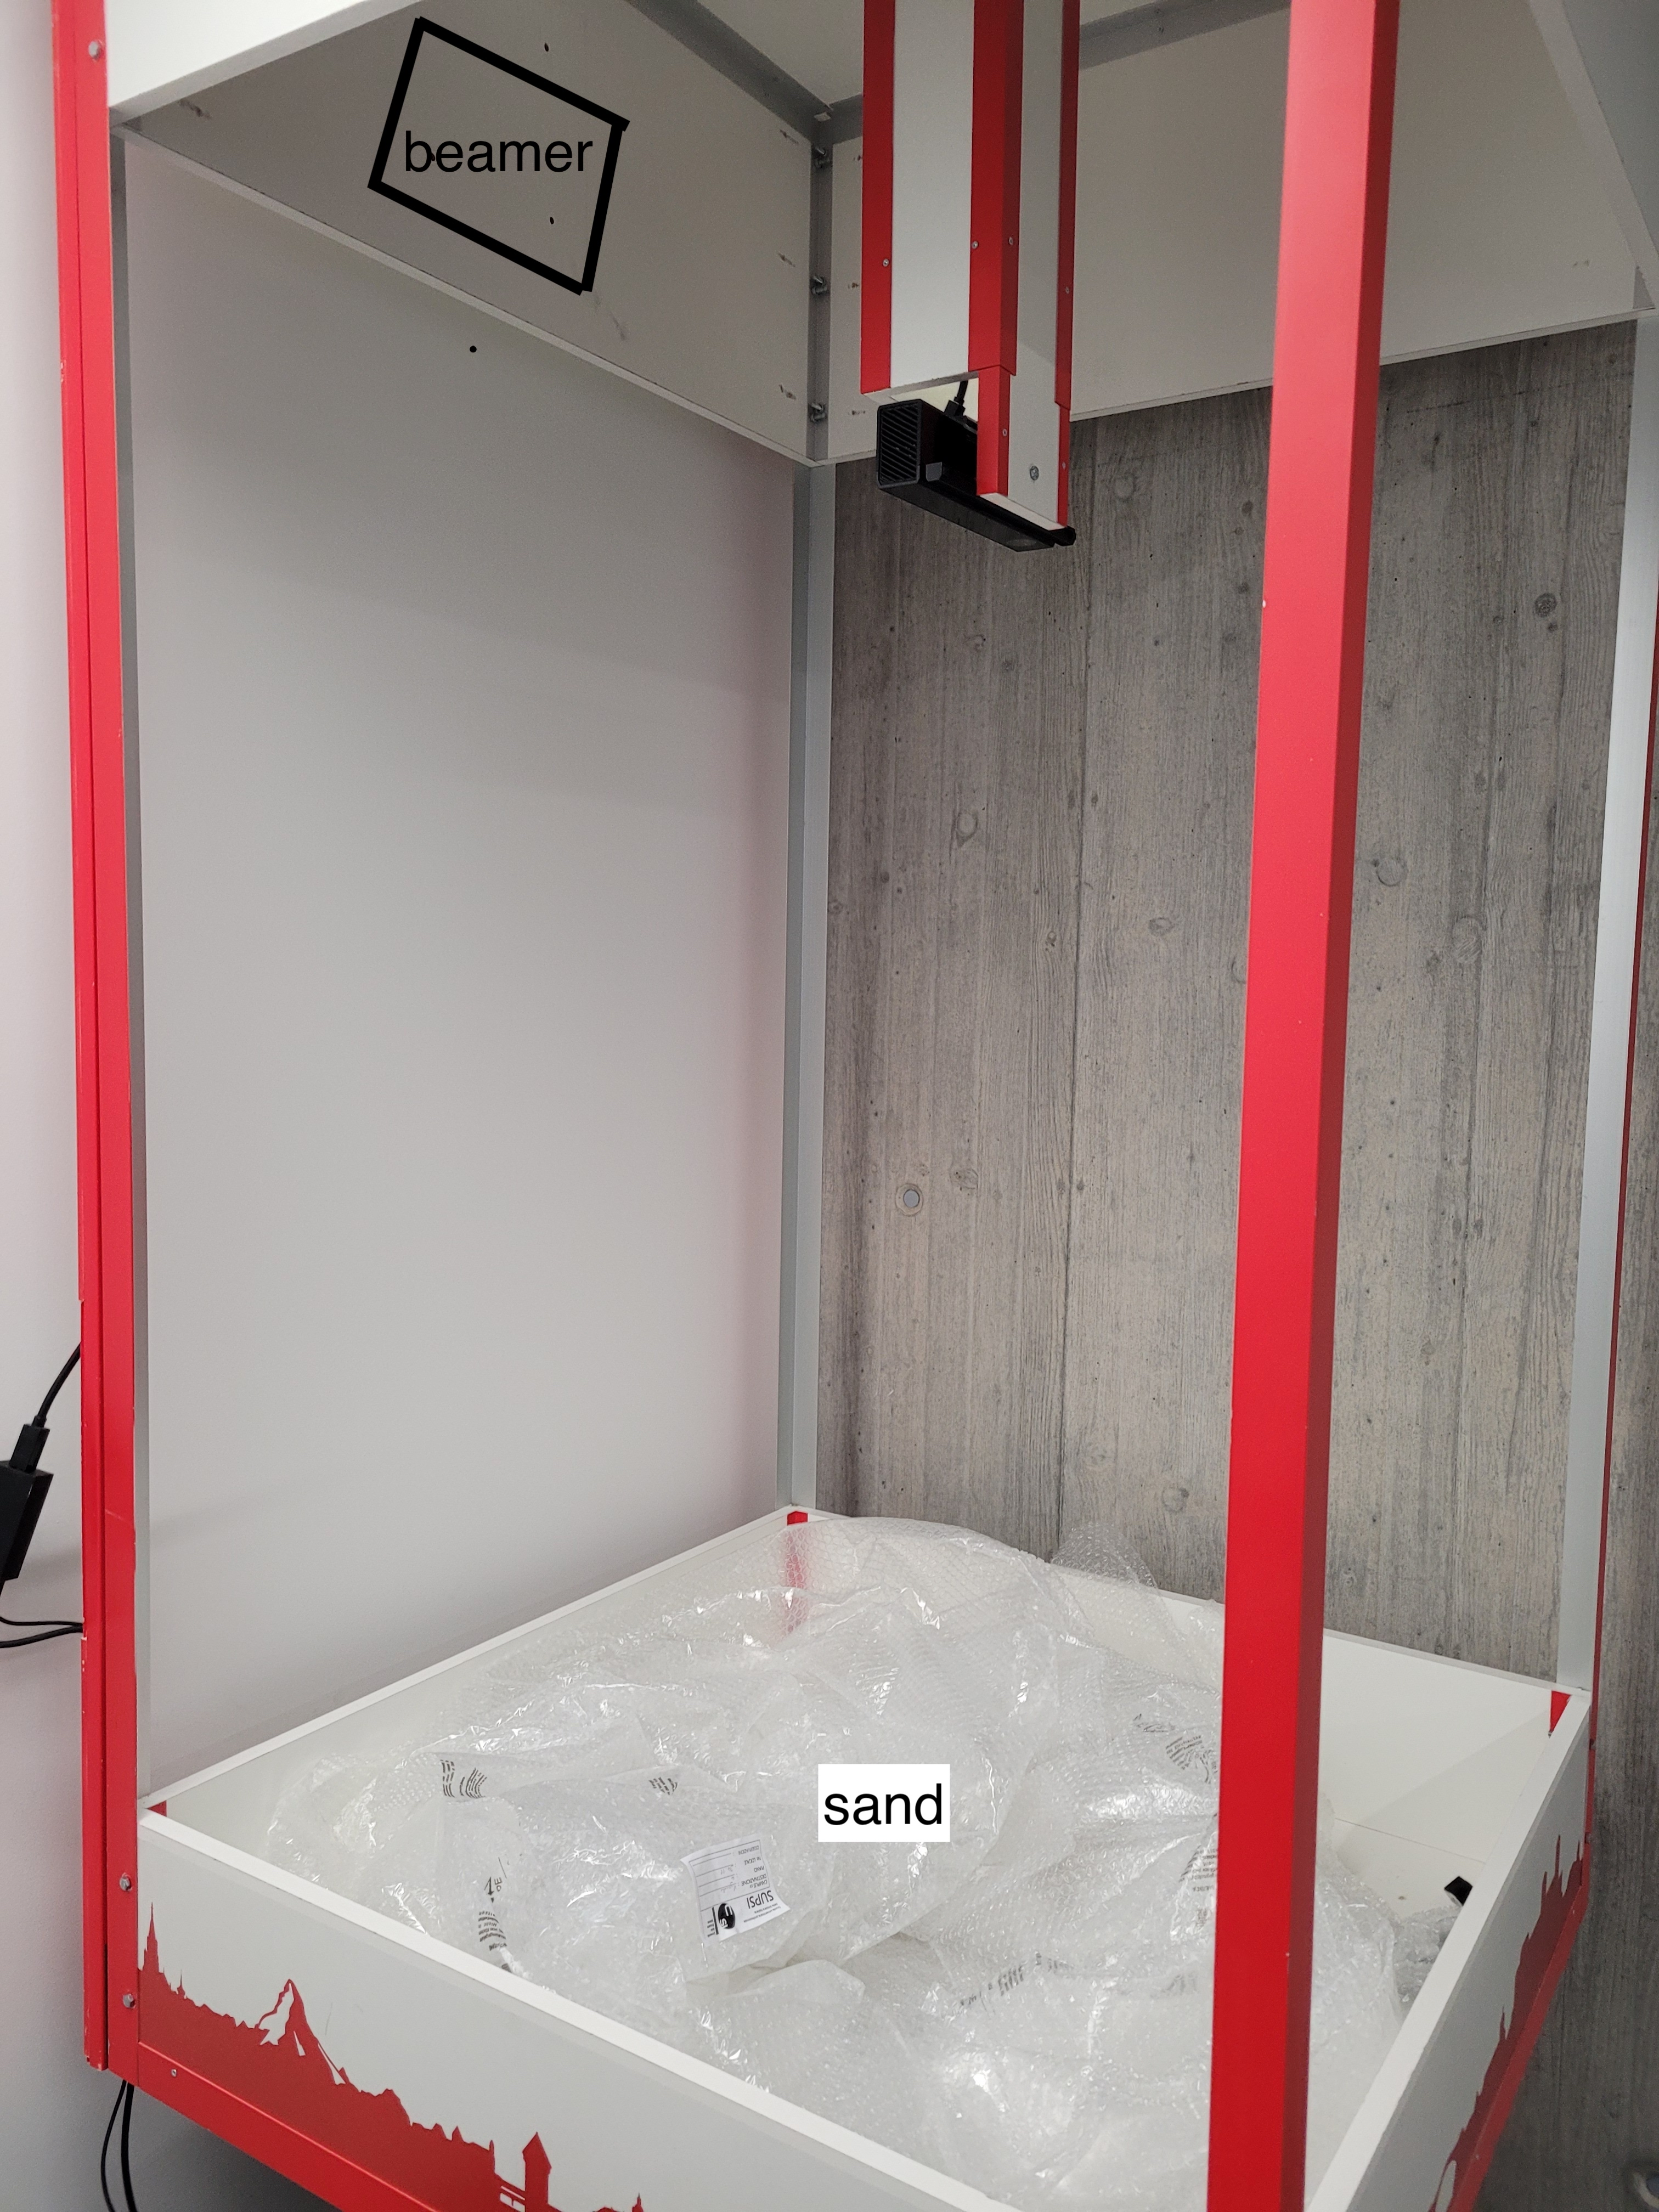
\includegraphics[width=0.85\textwidth]{img/sandbox.jpg}
	\caption*{Assembled sandbox with projector (1), Kinect (2) and its adapter (3), and PC (4)}
\end{figure}


\subsection{Startup}

ATTENTION: DO \textbf{NOT} connect the PC to the internet! The last Windows updates interfere with the functioning of the Kinect sensor.\\

Start the PC by pressing the power button and wait for the automatic start of the software. If the projector does not start automatically, press its power button.
In case of need, it is possible to start the software manually by clicking the \texttt{Launch sandbox} icon on the Desktop.\\

Once the software is open, the cows should start moving on the terrain. If this is not the case or the terrain remains always beige,
briefly press the \texttt{RESET} button on the front side of the PC and wait for the system to reboot.\\


\subsection{Shutdown}

Briefly press the power button of the PC to shut down the system and wait for the automatic shutdown of the projector.
DO \textbf{NOT} unplug the projector as long as the orange LED is flashing (cooling off)!!


\section{Usage}

Thanks to the Kinect sensor, the program recognizes the changes of height of the sand and automatically adapts the projected image.
The animals (cows or fishes, depending on the selected terrain) only walk on the surfaces that allow it, also adapting to the environment surrounding them.

\subsection{Frequent operations}

Change terrain: F5 $\rightarrow$ F1/F2/F3 $\rightarrow$ F5

Regulate height: F5 $\rightarrow$ Spacebar $\rightarrow$ U/J for the minimal height and I/K for the maximal $\rightarrow$ F5

Regulate image dimensions: F5 $\rightarrow$ Spacebar $\rightarrow$ see below for keys $\rightarrow$ F5

\newpage
\subsection{Useful keys}\label{sec:commands}

When in normal mode

\begin{tabular}{l l}
	ESC & exit              \\
	P   & save mesh         \\
	F5  & enter setup mode  \\
	-   & show terrain only \\
\end{tabular}

When in setup mode

\begin{tabular}{l l}
	F1      & select terrain 1 (mountains with cows)          \\
	F2      & select terrain 2 (lava)                         \\
	F3      & select terrain 3 (plains with fishes)           \\

	F5      & exit setup mode                                 \\

	1/2/3/4 & select corner                                   \\
	5       & resize terrain                                  \\
	6       & move terrain                                    \\

	W/A/S/D & move the terrain in the corresponding direction \\
	Shift   & slower movement                                 \\

	Spazio  & enable/disable preview                          \\

	9       & save calibration on disk                        \\
	0       & load calibration from disk                      \\

	U/J     & increase/reduce minimal height                  \\
	I/K     & increase/reduce maximal height                  \\
\end{tabular}

\section{Frequent problems}

\subsection{The image does not correspond to the sandbox dimensions}

Press the 0 button in setup mode to load the last saved configuration, then press the spacebar to see the preview.
The image can be regulated with the commands described in chapter \ref{sec:commands}. Press the F5 button to exit setup mode.\\

\subsection{The application suddenly closes}

The cow terrain (which is selected by default) is quite heavy and could cause the application to crash.
Should this happen, it is possible to select a less heavy terrain (fishes) by pressing the F3 button in setup mode.

\subsection{The image is bad quality or blurry}

Try regulating the focus of the projector by turning the ring around the lamp. In case of no change,
make sure the projector is \textbf{not} in 3D mode (menu $\rightarrow$ stereo $\rightarrow$ stereo mode).

\subsection{There are no cows, and the terrain remains beige}

Press the \texttt{RESET} button on the front side of the PC and wait for it to restart.


\section{Source code}\label{sec:code}

The source code for the application as well as the instructions to compile it can be found at \url{https://github.com/USI-Showroom/ARSandbox}.


\end{document}
